\documentclass[a4paper,12pt]{article}
\usepackage[utf8]{inputenc}
\usepackage[T2A]{fontenc}
\usepackage[russian,english]{babel}
\usepackage[pdftex]{graphics}
\DeclareGraphicsExtensions{.pdf,.png,.jpg}
\graphicspath{{pictures/}}
\begin{document}
\begin{center}
Санкт-Петербургский государственный политехнический университет
\\Кафедра компьютерных систем и программных технологий
\end{center}
\vspace*{10em plus .6em minus .5em}

\begin{center}
{\LARGEТелекоммуникационные технологии
\\Лабораторная работа №4
\\Аналоговая модуляция}
\end{center}

\vspace*{5em plus .6em minus .5em}
\begin{flushright}
Выполнил:\\студент гр.33501/4\\Курякин Д. А.\\Проверила:\\Богач Н.В.
\end{flushright}

\vspace*{15em plus .6em minus .5em}
\begin{center}
{\smallСанкт-Петербург
\\2018}
\end{center}
\pagestyle{empty}
\newpage
\pagestyle{plain}
{\bfseriesЦель}

Изучение амплитудной модуляции/демодуляции сигнала.

\section{Постановка задачи}

\begin{itemize}
	\item Сгенерировать однотональный сигнал низкой частоты.
	\item Выполнить амплитудную модуляцию (АМ) сигнала по закону $u(t)=(1+MU_mcos(\Omega t))+cos(\omega_0t+\phi_0)$ для различных значений глубины модуляции M. Используйте встроенную функцию
	MatLab ammod.
	\item Получить спектр модулированного сигнала.
	\item Выполнить модуляцию с подавлением несущей $u(t)=MU_mcos(\Omega t)cos(\omega_0 t+\phi_0)$. Получить спектр.
	\item  Выполнить однополосную модуляцию:
		
	$U(t)=U_mcos(\Omega t)cos(\omega_0t+\phi_0)+\frac{U_m}{2}\sum_{n=1}^{N}M_n(cos(\omega_0+\Omega_n)t+\phi_0+\Phi_0)$, положив n=1.
	\item Выполнить синхронное детектирование и получить исходный однополосный сигнал
	\item Рассчитать КПД модуляции
	
	$\eta_AM=\frac{U_m^2M^2/4}{P_U}=\frac{M^2}{M^2+2}$
\end{itemize}

\section{Теоретическое обоснование}

{\bfseriesМодуляция} -- это процесс преобразования одного или нескольких информационных параметров несущего сигнала в соответствии с мгновенными значениями информационного сигнала. В результате модуляции сигналы переносятся в область более высоких частот.

Использование модуляции позволяет:
\begin{itemize}
\item Согласовать параметры сигнала с параметрами линии;
\item Повысить помехоустойчивость сигналов;
\item Увеличить дальность передачи сигналов;
\item Организовать многоканальные системы передачи (МСП с ЧРК).
\end{itemize}

{\bfseriesАналоговая модуляция} является таким способом физического кодирования, при котором информация кодируется изменением амплитуды, частоты или фазы синусоидального сигнала несущей частоты.

При амплитудной модуляции для логической единицы выбирается один уровень амплитуды синусоиды несущей частоты, а для логического нуля - другой. Этот способ редко используется в чистом виде на практике из-за низкой помехоустойчивости, но часто применяется в сочетании с другим видом модуляции - фазовой модуляцией.

При частотной модуляции значения 0 и 1 исходных данных передаются синусоидами с различной частотой - f0 и f1. Этот способ модуляции не требует сложных схем в модемах и обычно применяется в низкоскоростных модемах, работающих на скоростях 300 или 1200 бит/с.

При фазовой модуляции значениям данных 0 и 1 соответствуют сигналы одинаковой частоты, нос различной фазой, например 0 и 180 градусов или 0,90,180 и 270 градусов.

\newpage

\section{Ход работы}
\begin{enumerate}
{\itemСгенерируем сигнал.
\center{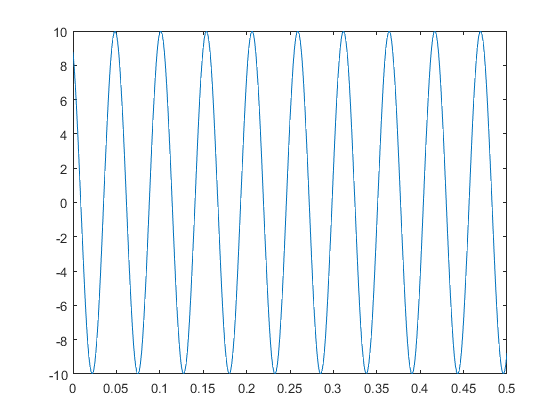
\includegraphics{./pictures/sig.png} \\ Рис.1 Сигнал}
\\}

{\itemВыполним амплитудную модуляцию, используя функцию ammod.
\center{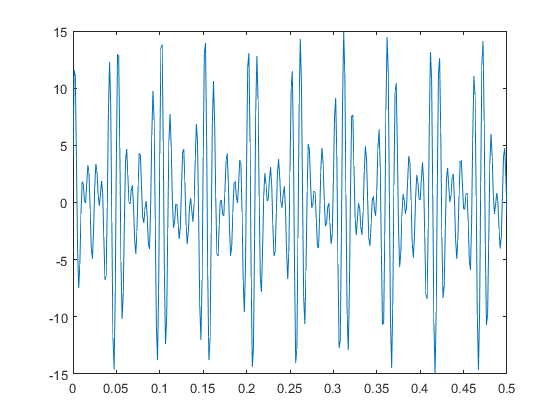
\includegraphics{./pictures/ammod.png} \\ Рис.2 Амплитудная модуляция}
\center{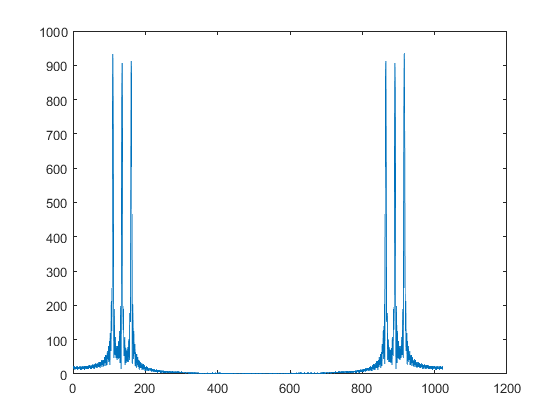
\includegraphics{./pictures/ammod_spec.png} \\ Рис.3 Спектр сигнала}
\\}

{\itemВыполним модуляцию с подавлением несущей.
\center{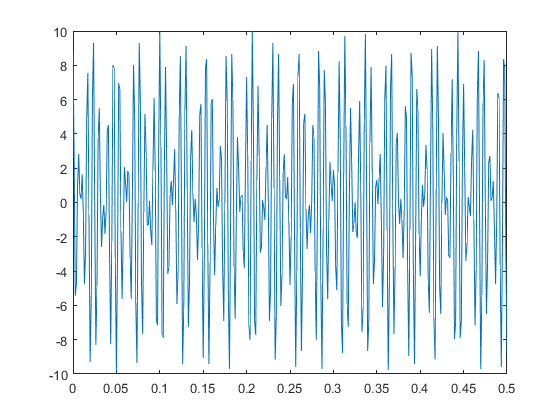
\includegraphics{./pictures/sub_mod.png} \\ Рис.4 Модуляция с подавлением несущей}
\center{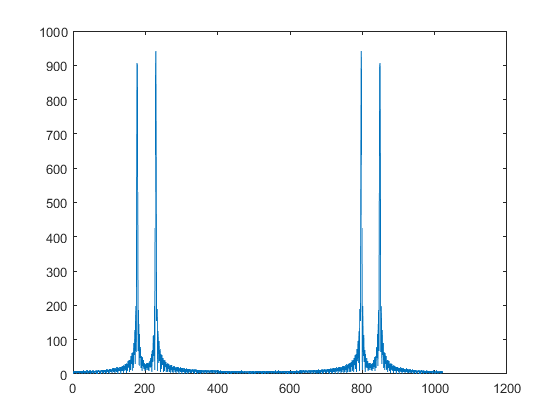
\includegraphics{./pictures/sub_mod_spec.png} \\ Рис.5 Спектр сигнала}
\\}

{\itemВыполним однополосную модуляцию, используя функцию ssbmod.
\center{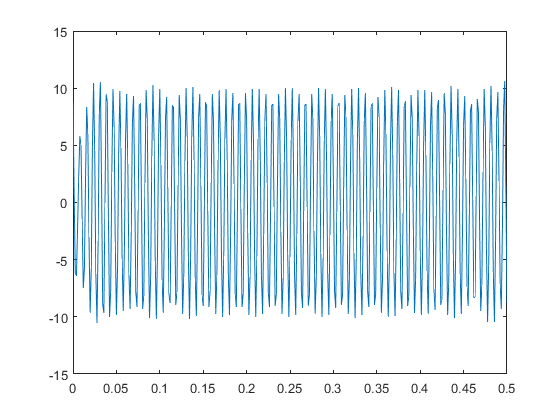
\includegraphics{./pictures/single_mod.png} \\ Рис.6 Однополосная модуляция}
\center{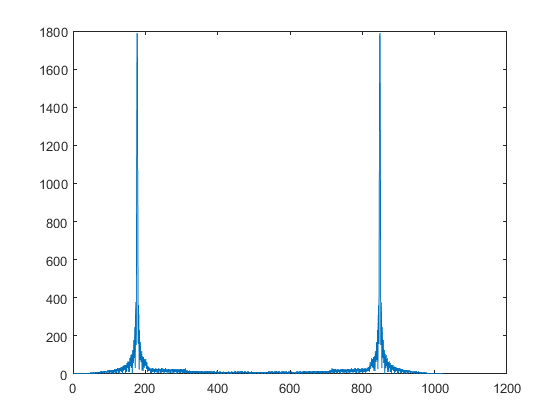
\includegraphics{./pictures/single_mod_spec.png} \\ Рис.7 Спектр сигнала}
\\}

{\itemВыполним синхронное детектирование и получим исходный однополосный сигнал.
\center{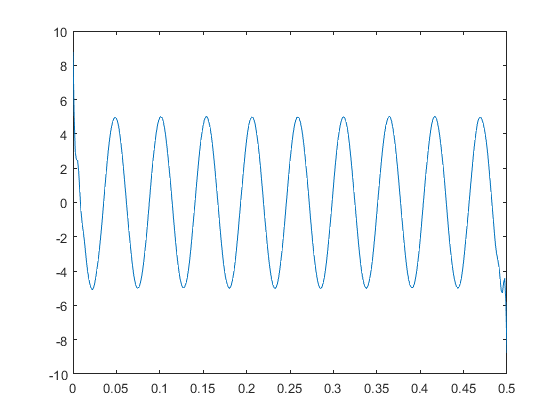
\includegraphics{./pictures/demod.png} \\ Рис.8 Сигнал после синхронного детектирования}
\center{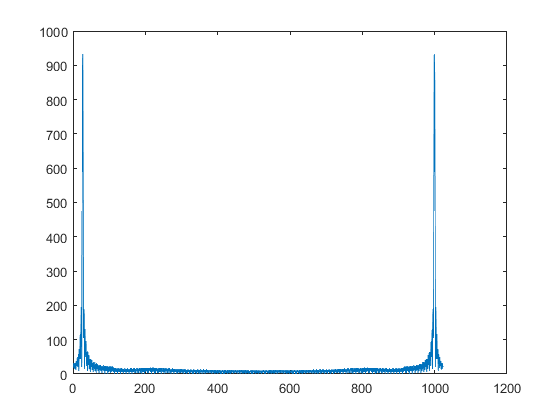
\includegraphics{./pictures/demod_spec.png} \\ Рис.9 Спектр сигнала}
\\}

{\itemНайдем КПД амплитудной модуляции.
КПД = 0.6667
\\}

\section{Вывод}

В ходе выполнения лабораторной работы исследована амплитудная модуляция/демодуляция сигнала. Основная мощность передаваемого информационного сигнала намного меньше мощности несущего колебания, поэтому амплитудная модуляция имеет низкий КПД. При подавлении несущей КПД модуляции равно 100\%.

\end{enumerate}
\end{document}
